\documentclass{article}

% Language setting
\usepackage[polish]{babel}

% Set page size and margins
\usepackage[a4paper,top=2cm,bottom=2cm,left=3cm,right=3cm,marginparwidth=1.75cm]{geometry}
\usepackage[T1]{fontenc}

% Useful packages
\usepackage{amsmath}
\usepackage{graphicx}
\usepackage{subcaption}
\usepackage[colorlinks=true, allcolors=blue]{hyperref}
\usepackage{float}
\usepackage{listings}

\title{CAD/CAE - zadanie 4}
\author{Iwo Szczepaniak}

\begin{document}
\maketitle

\section{Generowanie animacji}

\begin{verbatim}
function animate_terrain(terrain)
    fig = figure;
    frames = cell(1, ceil(360/10));
    frameIdx = 1;
    
    for angle = 1:10:360
        surf(terrain, 'EdgeColor', 'none');
        view(angle, 35);
        colormap(parula);
        lighting gouraud;
        material dull;
        
        drawnow;
        frame = getframe(fig);
        frames{frameIdx} = frame2im(frame);
        frameIdx = frameIdx + 1;
        
        clf(fig);
    end
    
    % Zapisywanie jako GIF
    filename = 'terrain_animation.gif';
    for idx = 1:length(frames)
        if isempty(frames{idx})
            continue;
        end
        [A,map] = rgb2ind(frames{idx},256);
        if idx == 1
            imwrite(A,map,filename,'gif','LoopCount',Inf,'DelayTime',0.1);
        else
            imwrite(A,map,filename,'gif','WriteMode','append','DelayTime',0.1);
        end
    end
end
\end{verbatim}

\section{Mapa wysokości}

\begin{figure}[H]
    \centering
    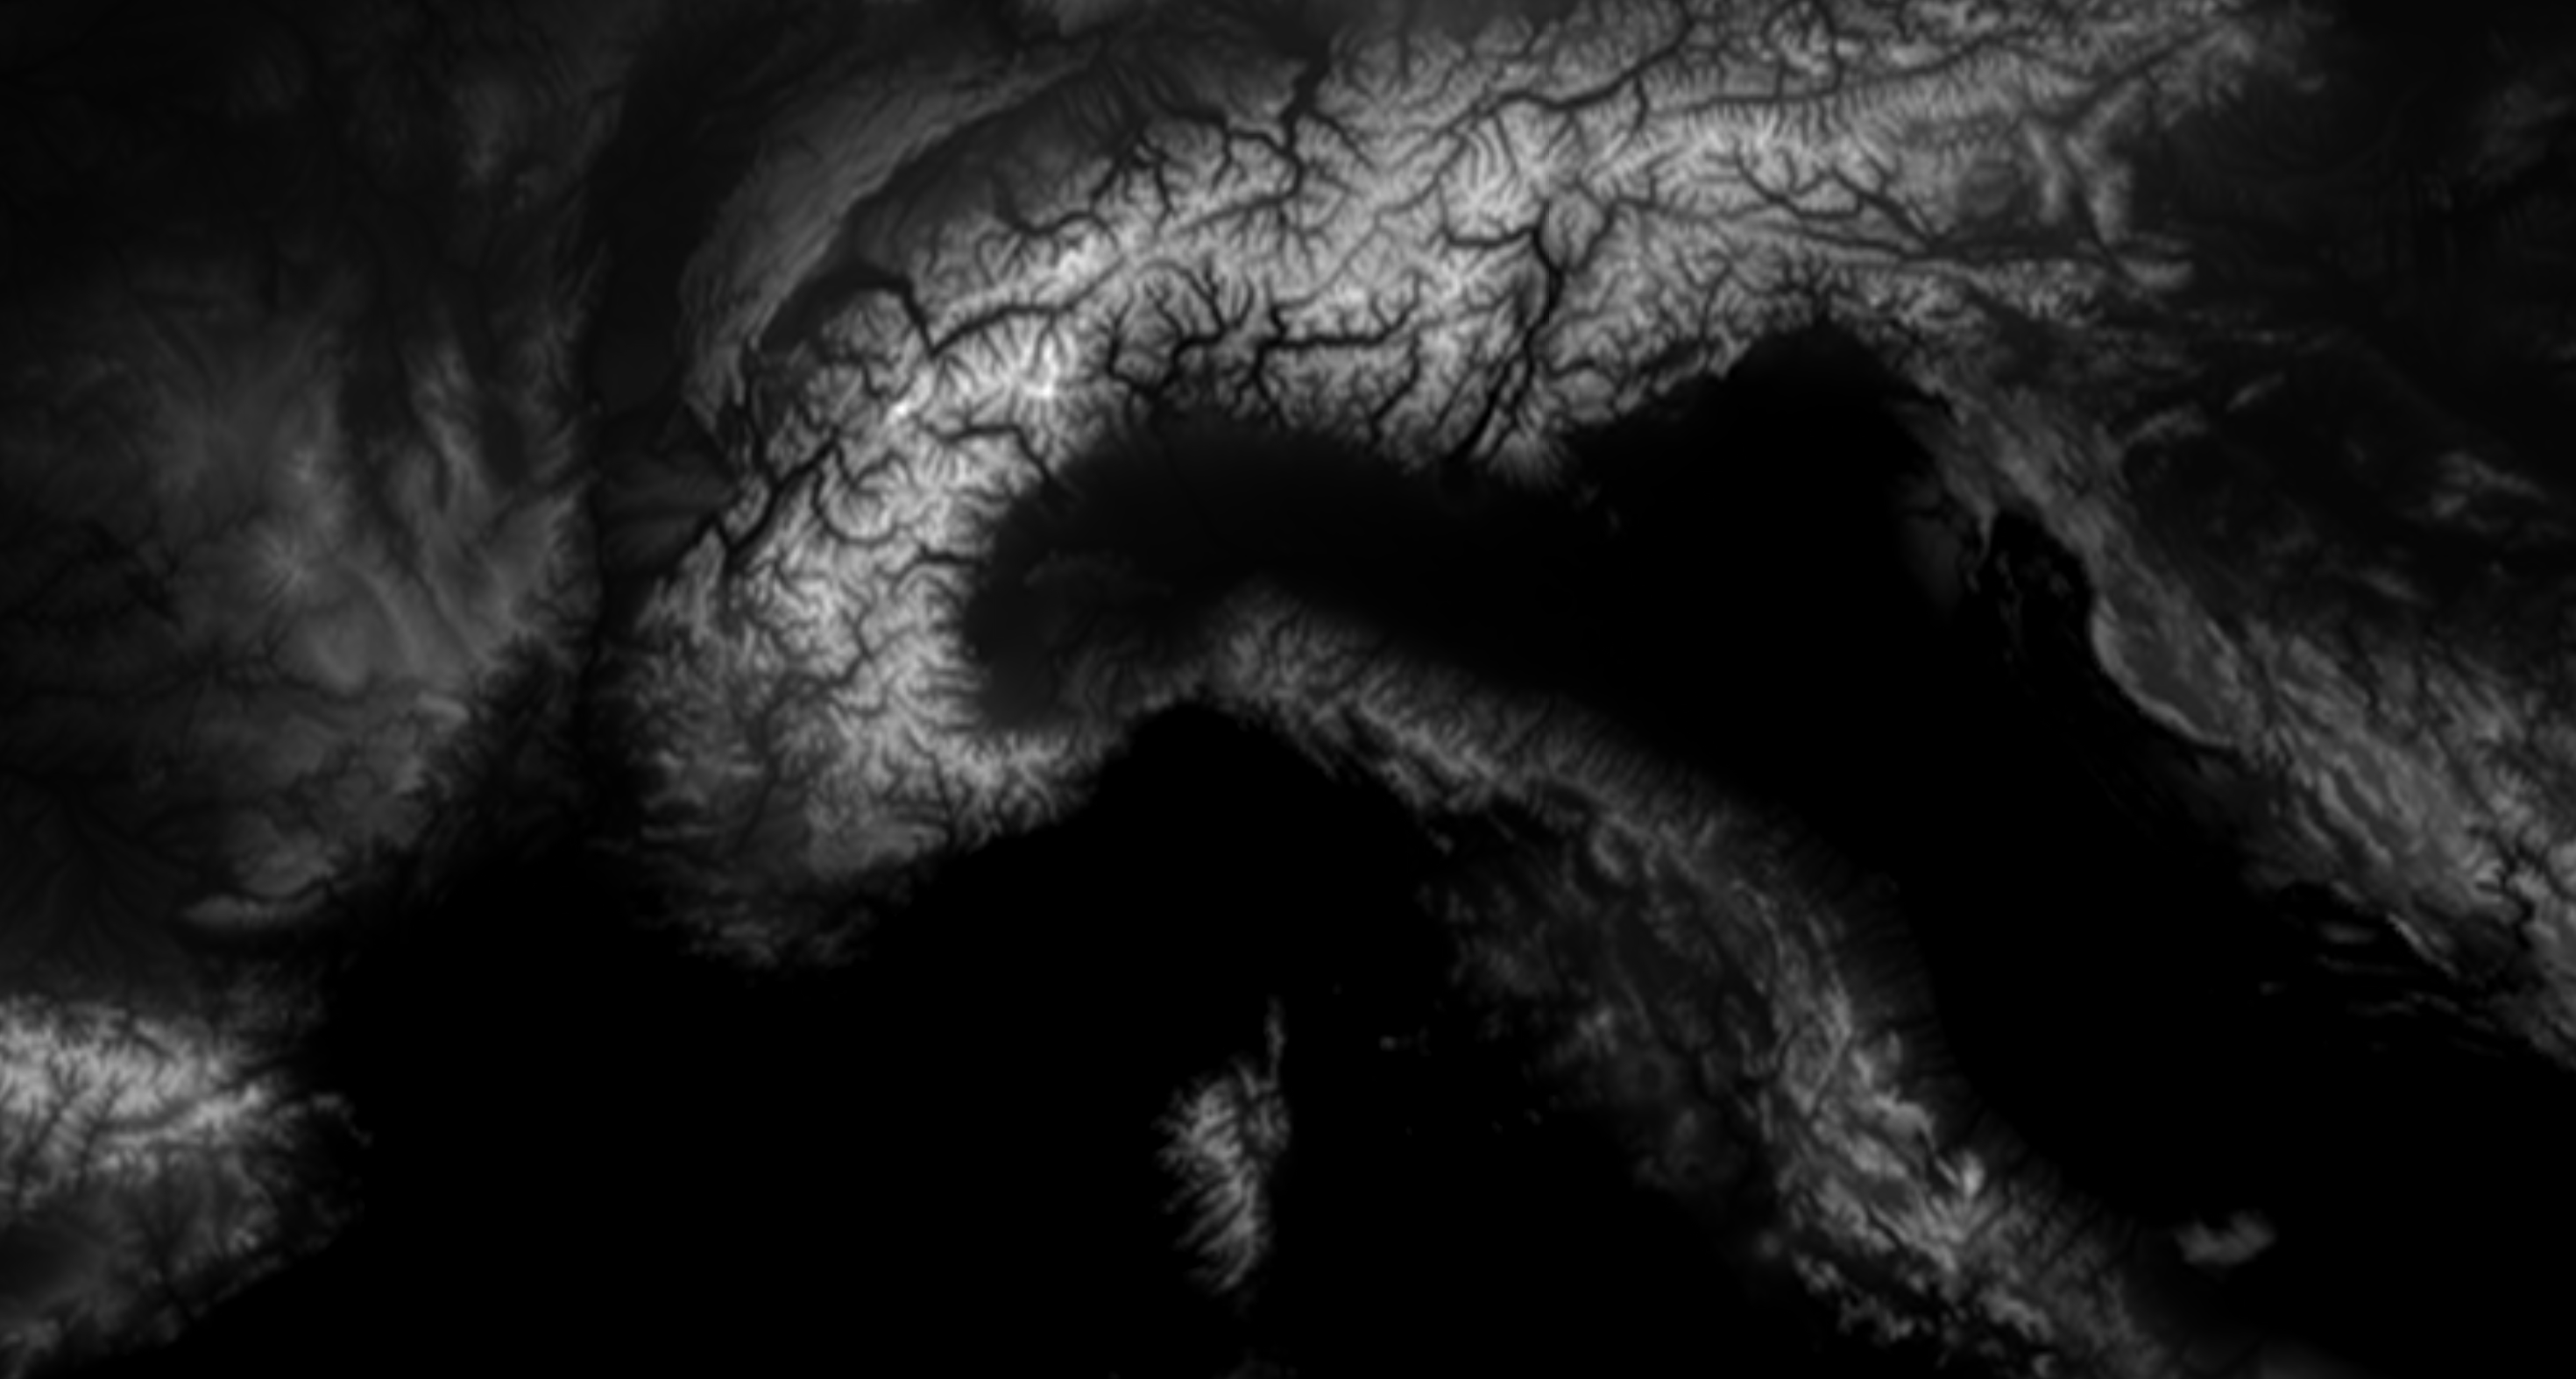
\includegraphics[width=0.8\linewidth]{download.png}
    \caption{Mapa wysokości północnych Włoch \newline - dane wejściowe do bitmap\_terrain}
    \label{fig:height-map}
\end{figure}


\begin{figure}[H]
    \centering
    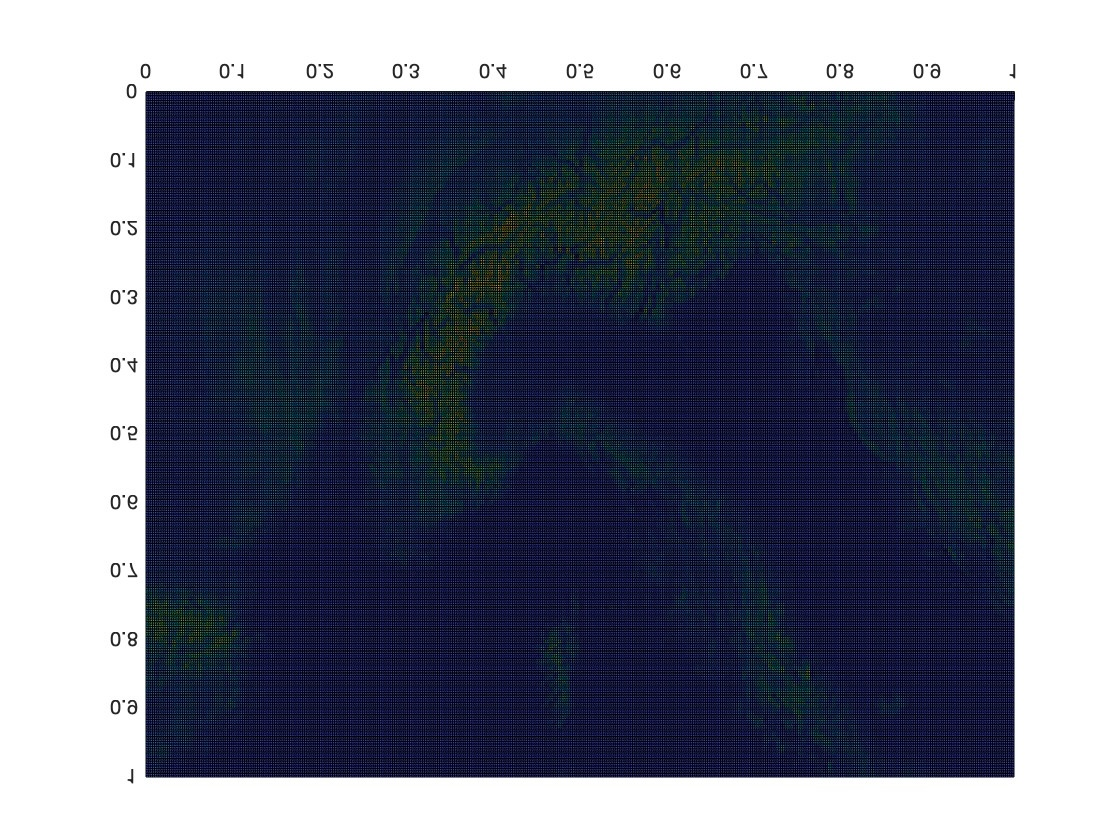
\includegraphics[width=0.95\linewidth]{terrrain_map.jpg}
    \caption{Bitmapa wysokości terenu \newline - dane wejściowe do rysowania spline`a}
    \label{fig:height-map}
\end{figure}

\section{Wizualizacje terenu}

\subsection{Widok 2D}
\begin{figure}[H]
    \centering
    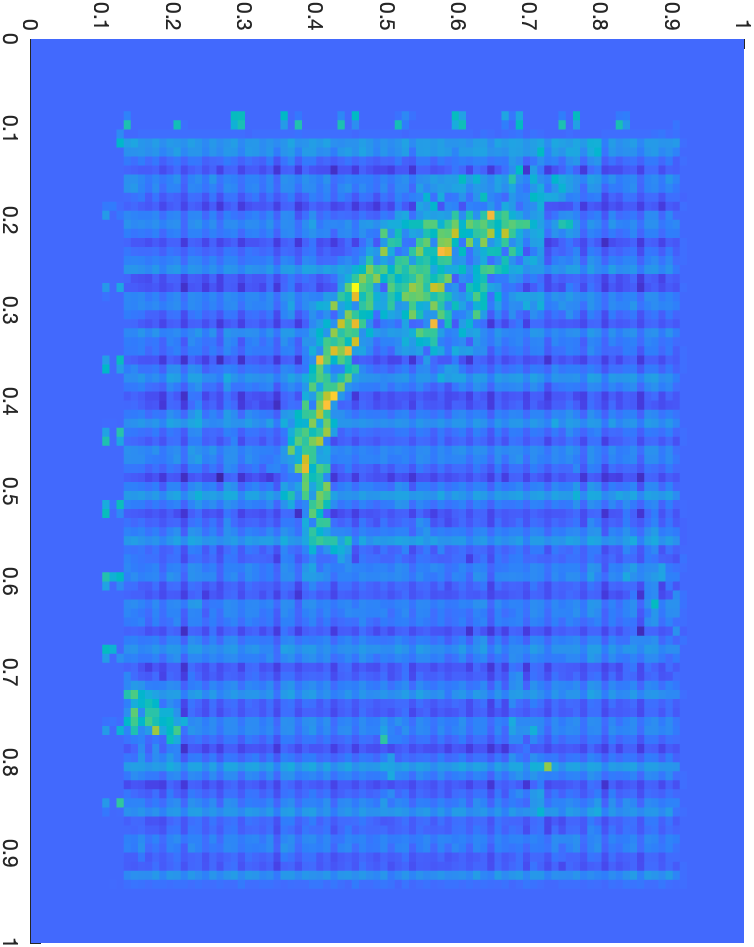
\includegraphics[width=0.7\linewidth]{2D.png}
    \caption{Widok z góry wygenerowanego terenu}
    \label{fig:2d-view}
\end{figure}

\subsection{Widoki 3D}
\begin{figure}[H]
    \centering
    \begin{subfigure}[b]{0.45\textwidth}
        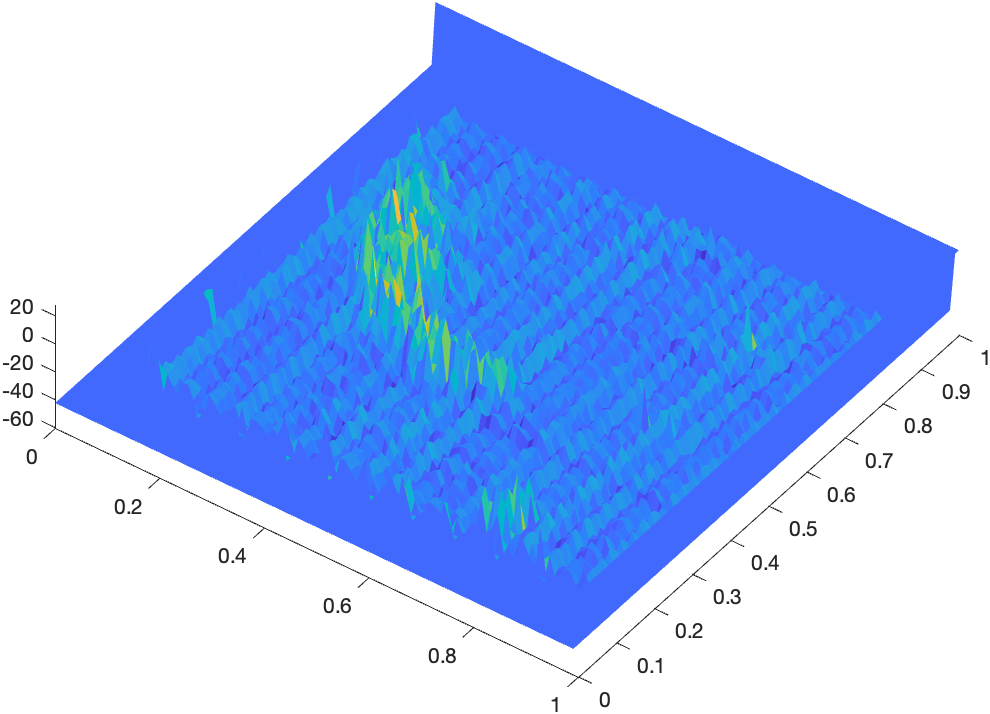
\includegraphics[width=\textwidth]{3D_1.png}
        \caption{Widok z perspektywy 1}
    \end{subfigure}
    \begin{subfigure}[b]{0.45\textwidth}
        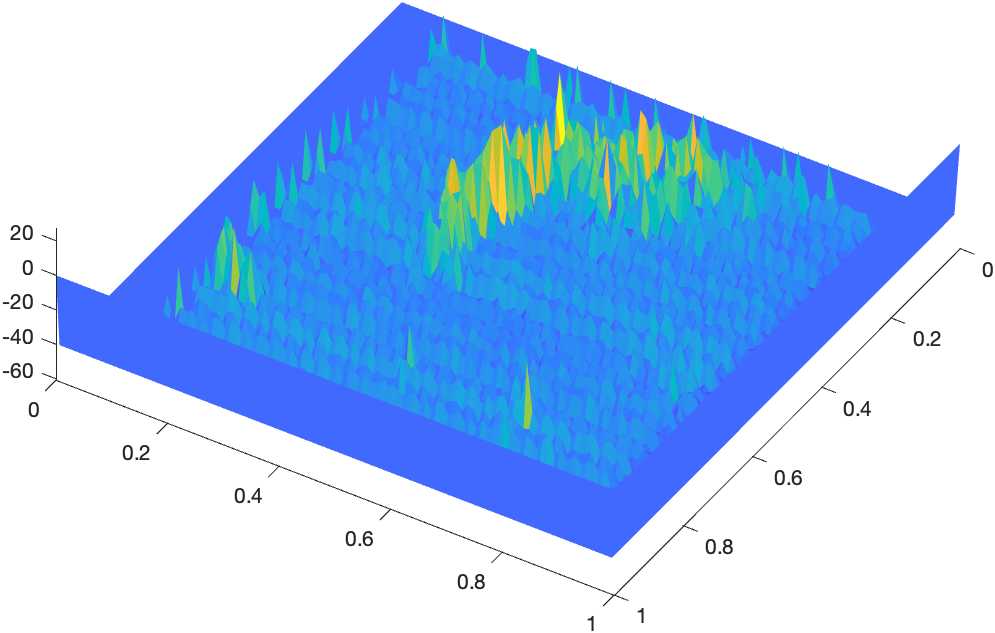
\includegraphics[width=\textwidth]{3D_2.png}
        \caption{Widok z perspektywy 2}
    \end{subfigure}
    \begin{subfigure}[b]{0.45\textwidth}
        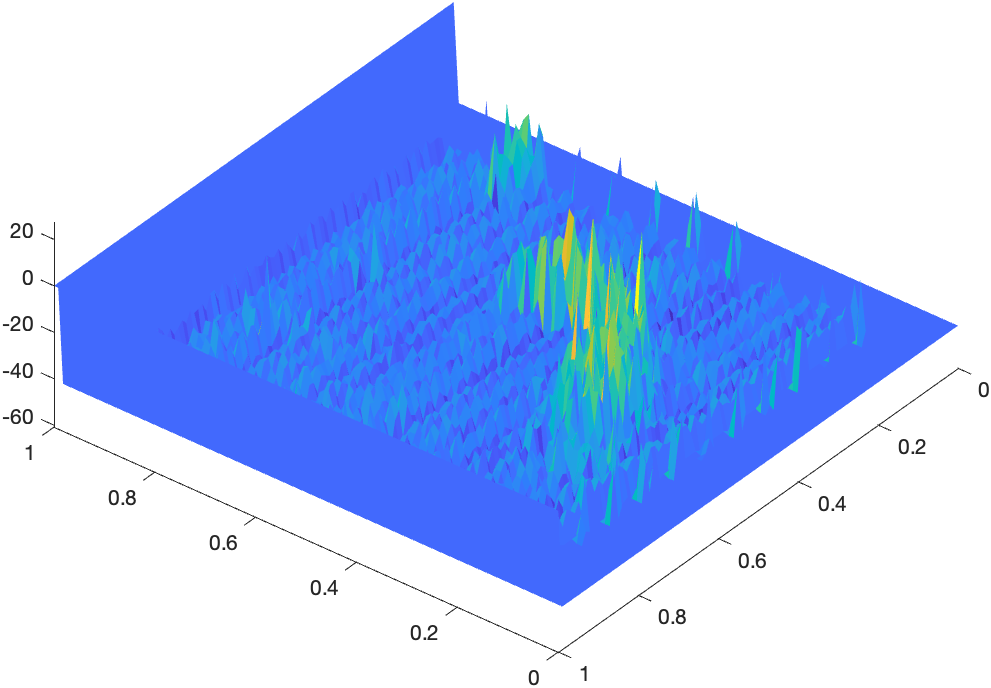
\includegraphics[width=\textwidth]{3D_3.png}
        \caption{Widok z perspektywy 3}
    \end{subfigure}
    \begin{subfigure}[b]{0.45\textwidth}
        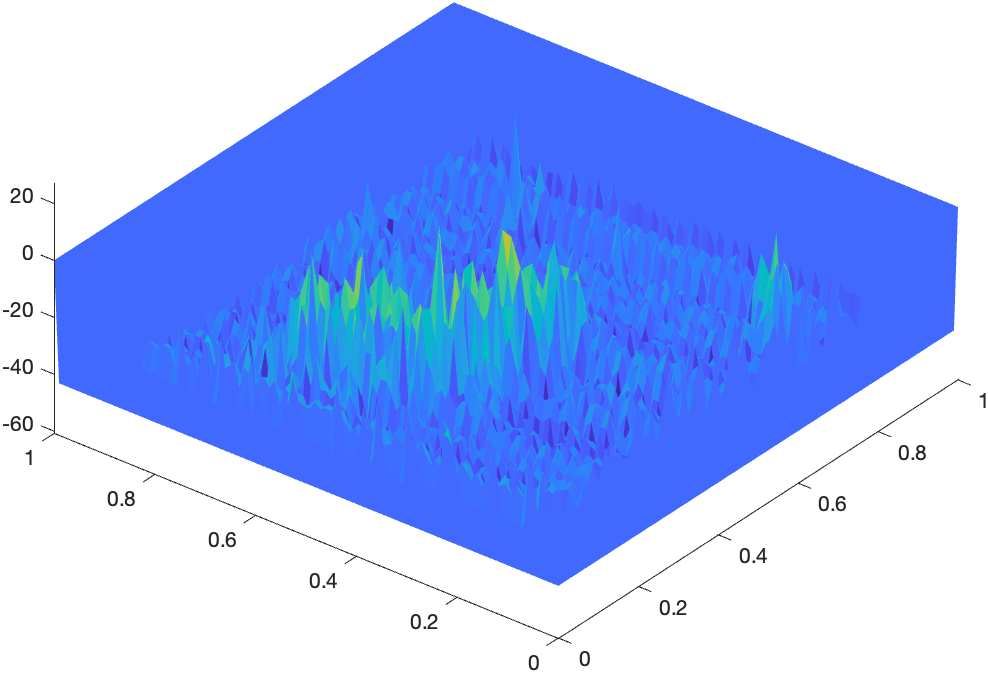
\includegraphics[width=\textwidth]{3D_4.png}
        \caption{Widok z perspektywy 4}
    \end{subfigure}
    \caption{Różne perspektywy wygenerowanego terenu 3D}
    \label{fig:3d-views}
\end{figure}


\end{document}